\documentclass[a4paper, 12pt]{scrartcl}

\usepackage[english]{babel}
\usepackage[utf8]{inputenc}
\usepackage{amsmath}
\usepackage{geometry}
\usepackage{caption}
\usepackage{graphicx}
\usepackage[colorinlistoftodos]{todonotes}
\usepackage{hyperref}
\usepackage{booktabs}
\usepackage{cleveref}
\usepackage{listings}
\usepackage{listings-golang}
\usepackage{makecell}
\usepackage{sectsty}
\usepackage{comment}
\usepackage{multicol}

\let\bold\textbf
\setlength\parindent{0pt}
% \todo[inline]{Add diagram here}

\title{\vspace{10mm}CS628 Assignment 1 \\ $2018\text{-}19$  II Semester \\ \vspace{1cm} \textbf{Design Report for Secure Key-Value File Sharing}}
\subtitle{\vspace{4mm}\includegraphics[width=\textwidth, height=10cm]{images/cs628.png}\vspace{20mm}}
\author{Aniket Pandey $(160113)$ \hspace{5mm} $\cdot$ \hspace{5mm} Ashish Kumar $(160160)$ \\ \textit{B.S MTH} \hspace{45mm} \textit{B.Tech CSE}}
\date{\today}

\geometry{
a4paper,
total={180mm,260mm},
left=15mm,
top=15mm,}

%\sectionfont{\fontsize{15}{15}\selectfont}
%
%\title{%
%   \includegraphics[width=13cm, height=5cm]{cs628.png}
%}

\begin{document}
\clearpage\maketitle
\thispagestyle{empty}
\newpage

%\begin{center}
%	\includegraphics[width=13cm, height=5cm]{cs628.png}
%\end{center}

\section{A simple, but secure client}
\textbf{Purpose:} To maintain Confidentiality and Integrity of data without any regards to Availability.
\textbf{NOTE:} \textit{KeyAddr} field in every struct to protect against key-value-swap attack.

\begin{multicols}{2}

\begin{center}
	\textbf{USER Structure}
\end{center}

\begin{center}
	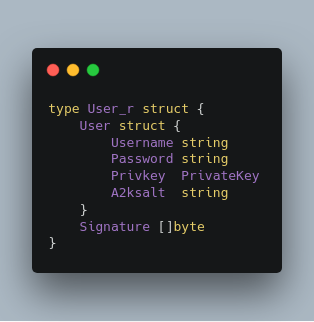
\includegraphics[width=7cm, height=6cm]{images/user.png}
\end{center}

\columnbreak

\begin{center}
	\textbf{INODE Structure}
\end{center}

\begin{center}
	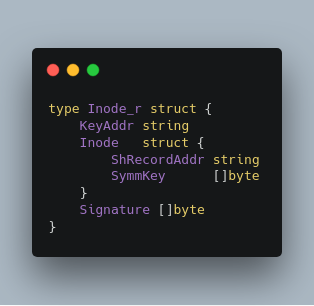
\includegraphics[width=7cm, height=6cm]{images/inode.png}
\end{center}

\end{multicols}

\subsection{InitUser (username string, password string)}
\begin{enumerate}
	\itemsep0em

	\item Obtain $key = Argon2Key("<password>+<username>", "<username>+user", 10)$. This will generate a 36 character key. This is where the value (User data) will be stored.
	\item Generate an RSA Key-pair. Push the public key to the Public Key Server. Store the Private Key along with other fields in User\_r struct.
	\item Generate a new $key = Argon2Key("<username>+<password>", "<username>", 10)$ for symmetric encryption. Use this key to sign \textit{User\_r.User} with HMAC scheme, store the signature in \textit{User\_r.Signature}. Encrypt the json-marshalled \textit{User\_r} struct data with AES-Cipher Feedback Mode using the same key as above.
	\item Call $DatastoreSet(key, ciphertext)$ to publish the encrypted User information in Data Server.
\end{enumerate}

\subsection{GetUser (username string, password string)}
\begin{enumerate}
	\itemsep0em

	\item Get the "key" using above Argon2Key invocation. Errors suggest either incorrect username or password. Calculate the key for CFBDecrypter(), and obtain the decrypted \textit{User\_r} structure.
	\item Check HMAC hashes of $User\_r.User$ and $User\_r.Signature$ for any tampering. If all checks are satisfied, return the $User\_r.User$ structure.
\end{enumerate}

\subsection{(User) StoreFile (filename string, data []byte)}
\begin{enumerate}
	\itemsep0em
	\item Obtain $key = Argon2Key(<password>+<filename>", "<username>+<filename", 10)$. This will generate a 36 character key. This is where the Inode structure for "Username"-"Filename" will be stored (Refer to the figure).
	\item Generate a random address (key) and AES-CFB key for storing and encrypting SharingRecord\_r structure respectively. Fill the Inode structure. Sign it using Author's Private key and store RSA signature in $Inode\_r.Signature$. Encrypt $Inode\_r$ with Author's Public key. Push (key, encrypted Inode\_r) to Data Server.
	\item Check if a $SharingRecord\_r$ structure exists. If it exists, delete all the existing data blocks and write the new data. Else, initialize a new $SharingRecord\_r$ object.
	\item Again generate a random address (key) and AES-CFB key for storing and encrypting the $Data\_r$ structure. Store these in the relevant fields of SharingRecord structure. Sign with a predecided HMAC key and store in $SharingRecord_r.Signature$ field. Encrypt the Structure with the key decided at $Inode\_r$ and push to Data Server.
	\item Store the "data" at the "key" generated above, Encrypt it with CFBEncrypter() method. Sign it and store the data at the "key". Push to Data Server and return. 
\end{enumerate}

\begin{multicols}{2}

\begin{center}
	\textbf{SharingRecord Structure}
\end{center}

\begin{center}
	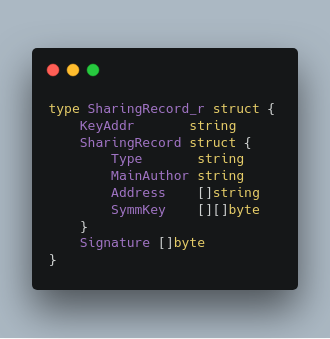
\includegraphics[width=7cm, height=6cm]{images/sharing.png}
\end{center}

\columnbreak

\begin{center}
	\textbf{DATA Structure}
\end{center}

\begin{center}
	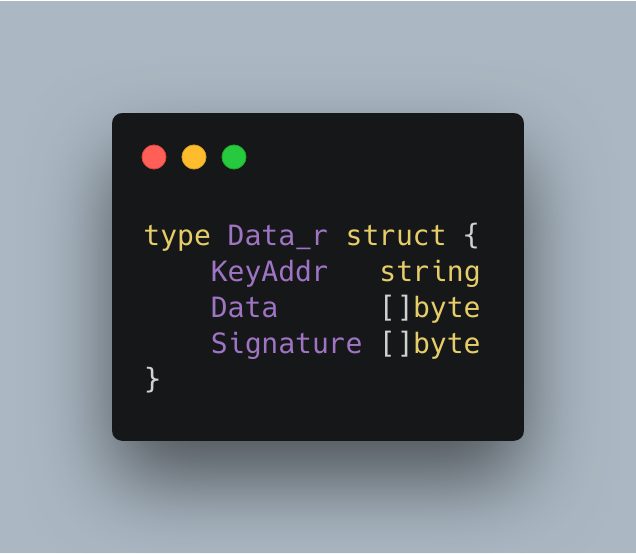
\includegraphics[width=7cm, height=6cm]{images/data.png}
\end{center}

\end{multicols}

\subsection{(User) LoadFile (filename string)}
\begin{enumerate}
	\itemsep0em
	\item Follow the method given in StoreFile() to reach, decrypt and verify the signature of the $SharingRecord\_r$ structure corresponding to "filename".
	\item Loop over the list of addresses of data chunks (via indirect pointers), decrypt and verify the HMAC signatures of each, reconstruct the entire data as a single byte array and return it.

\end{enumerate}

\subsection{(User) AppendFile (filename string, data []byte)}
\begin{enumerate}
	\itemsep0em
	\item Follow the method given in LoadFile() to reach, decrypt and verify the signature of the $SharingRecord\_r$ structure corresponding to "filename". 
	\item Create a new $Data\_r$ block and append its generated encryption key and address to the appropriate list of keys and signatures in SharingRecord structure. Push the block to DataStore and return.
	\item \textbf{NOTE:} We are not verifying the integrity of previous data blocks during AppendFile(), considering the unnecessary overhead of re-encryptions/decryptions.
\end{enumerate}

\section{Sharing and revocation}

\subsection{(User) ShareFile (filename string, recipient string)}
\begin{enumerate}
	\itemsep0em
	\item Follow the method given in LoadFile() to reach, decrypt and verify the signature of the $SharingRecord\_r$ structure corresponding to "filename".
	\item $collected\_info = Inode\_r.Inode.(Symmkey + ShRecordAddr)$. Recieve the Public key of receiver from the Public Key Server.
	\item $sharing = PubKey_{recipient}(PrivKey_{user}(Hash(collected\_info)) + (collected\_info))$, to maintain confidentiality and integrity in case of a \textbf{Man in the Middle attack} while sharing the message offline. Where $PrivKey_{user}(Hash(collected\_info))$ is the signature of $collected\_info$.
\end{enumerate}

\subsection{(User) ReceiveFile (filename string, sender string, msgid string)}
\begin{enumerate}
	\itemsep0em
	\item Decrypt "msgid" using Private Key of User, verify the integrity using Public Key of Sender. Obtain the Address and "key" for CFB-Decryption of SharingRecord structure of the concerned data(value) and proceed ahead.
	\item Create an Inode for the receiver user using Argon2Key, with the method described in StoreFile(). Store the info in the Inode, store the RSA signature and encrypt $Inode\_r$ structure with Public key of User. Return.
\end{enumerate}

\subsection{(User) RevokeFile (filename string)}
\begin{enumerate}
	\itemsep0em
	\item Go to the SharingRecord structure corresponding to "filename". \textbf{IMP:} After verifying the integrity, check if the User is \textbf{Original-Author} of the "filename". If not, return an error.
	\item If so, from the Inode of original author, change the encryption key and the address of $SharingRecord\_r$ structure and re-encrypt it with a new key. Similarly, change the address of the actual data ($SharingRecord\_r.Address$).
	\item Iterate over all data-blocks and re-encrypt them with fresh symmetric keys. Also, store each of them at new addresses. Store these new keys and addresses in the corresponding $SharingRecord\_r$ structure. \textbf{NOTE:} This is to prevent any further misuse by a distrusted user who knows the original keys and addresses of data blocks.
\end{enumerate}

\end{document}
